%!TeX program=pdflatex
%!TeX encoding=utf8
%!TeX spellcheck = en_US
%!TeX root = ../../messageVortex.tex

\part{Results}
To verify the hypothesis made in this paper, and to analyse properties of the protocol in a real world scenario a library was implemented in Java which was capable of handling all message packets and the routing stack as a whole. The following paragraphs describe the protocol developed in general as a generic approach. Appendix \ref{app:rfcMessageVortexMain} gives the full ASN.1 representation of the protocol. 

It is important to notice that ASN.1 has no mean to express encrypted structures. Due to this fact we defined all encrypted fields as \verb|OCTET STRING|. 

The protocol is defined int the ASN.1 to support onionized information in an unencrypted form. This is meant for debugging purposes only. At no point should this possibility be used in a production environment.

The protocol described in the next chapter is independent from routing. We built a blending layer for SMTP. Layers for other protocols such as XMMPP may be built similarly. The protocol may be extended by adding blending layers and their addressing schemes.

The Protocol outlined here is the final product and has undergone many development cycles. A lot of really useful features and capabilities such as a mechanism analoguous to the SMTP received headers were dropped as they were very useful but threatened security or anonymity.

\chapter{Protocol Overview}
The MessageVortex protocol described here is an onionizing protocol for asynchronus data transfer. The protocol itself is embbeded into a carrier protocol as binary information to avoid easy detection and make it hard to block traffic without blocking other legitimate traffic.

The Protocol implementation is described in the RFC document in \ref{app:rfcMessageVortexMain}. It contains all necessary information to build the protocol. It is published on the website \url{https://messagevortex.net/} and on the official IETF channels. Beside the RFC document additional documents and a reference may be found.

The data transferred is passed thru a number of mixes. The builder of a routing block (normally the sender) decides upon the following attributes:
\begin{itemize}
	\item Hops for the message and all decoy traffic.
	\item Timing behaviour respectively speed of the message.
	\item Decoy traffic generation.
	\item Set of possible recipients.
\end{itemize}

These decisions are compiled into a routing block structure which is onionized. This routing block may then be used to transfer a message of almost any size. This message is then sent to the involved mixes.

A mix may be just an intermediate station or the final target of a message. Only the recipient of a message is able to tell whether a message was intended for him or not. Any mix does a certain number of operations on a message. Considering the message, the timing and the operations applied a mix may extract the following informations:

\begin{itemize}
	\item IP of the sending mix.
	\item Size of the message received.
	\item Size of all processed sub blocks.
	\item Arrival time of a message.
	\item Ephemeral identity a message belongs to (ephemeral pseudonym to the routing block builder).
	\item Validity time of the message on the node.
	\item Operations applied to the message.
	\item Size of all blocks sent.
	\item IPs of the receiving mixes.
\end{itemize}

A mix always applies the operations requested in the building instructions to the received data. If this is not done properly the message may fail to transfer to its final destination. 

The operations to be applied on a message are chosen in such a way that they may or may not generate decoy traffic. This guarantees that a valid message may not be identified on the operations applied to the message.

Redundancy may be built in a routing block as well as progress indication.

In the taxonomy of \cite{Shirazi2018} this protocol would be classified as follows:

\begin{itemize}
	\item Network topology: full
	\item Network connection direction: unidirectional
	\item Network connection syncronization: asynchronous
	\item Network symmetry roles: hybrid
	\item Network symmetry topology: flat
	\item Network symmetry decentrallization: fully decentralized
	\item Routing network view: partial
	\item Routing updating: Event based
	\item Communication routing type: source routed\footnote{Only partially correct, as the routing block builder decides on the route. This builder is not necesarily identical to the sender.}
	\item Communication scheduling: fair
	\item Communication node selection determinism: probabilistic
	\item Communication node selection set: user-based
	\item Communication node selection selection probability: uniform
	\item Performance latency: high
	\item Performance communication mode: message-based
	\item Performance implementation: yes
	\item Performances code availability: yes
	\item Performance context: email, messaging
\end{itemize}

\section{Vortex Message}
The outline in figure \ref{fig:messageOutline} is a simplified view onto the message block of MessageVortex.

\begin{figure*}[ht]
	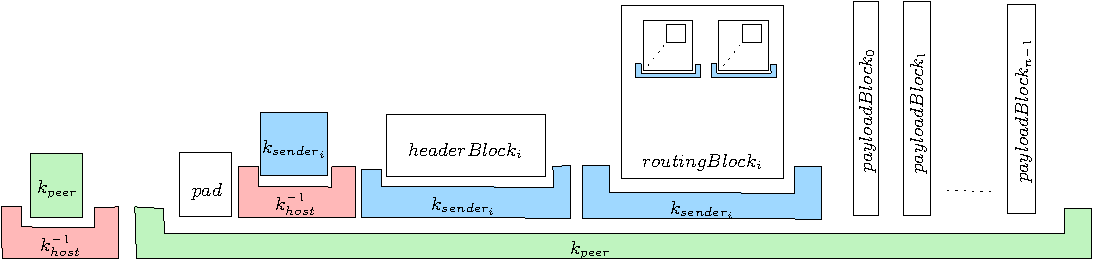
\includegraphics[width=\textwidth]{inc/blockLayoutSimplified}
	\caption{Simplified message outline}
    \label{fig:messageOutline}
\end{figure*}

A vortex message is a message passed from one mix to another this message may or may not contain any valuable information. The message itself is embedded as binary data into a transfer protocol. Every Mix may decide for himself what kind of protocols and embedding mechanisms are supported.

A vortex message is always built out of these blocks:
\begin{itemize}
	\item header
	\begin{itemize}
		\item Encrypted message key.\\
			  Contains symmetrical key for decryption of follow up header information and payload blocks. Encrypted with host identity public key.
		\item Identity and ``proof of work'' information\\
		      Contains Requests, Proof of work sections, and header key
	\end{itemize}
	\item Encrypted payload blocks (encrypted with header key)
	\begin{itemize}
		\item Routing blocks (encrypted with message key)
		\begin{itemize}
			\item Next hop timing instructions
			\item Next hop routing blocks (encrypted)
			\item Next hop header
			\item Message build instructions.
			\item Next hop header key and spec.
			\item Next hop blending instructions.
		\end{itemize}
		\item Payload chunk blocks
	\end{itemize}
\end{itemize}

It is important to note that there are two symmetrical keys involved in encrypting and decrypting message headers. This is not a flaw in the protocol but necessary. 

The first key which is in a Vortex message is the message key. This key is only accessible with the private key of the node receiving the message. It allows decryption of the routing blocks and the header information. The sender of a message block is therefore not able to tell if a message contains one or more routing blocks. It is important to note that no other node should have access to this information. 

The second key is the header key located in the encrypted header. This key was chosen by the creator of the routing block containing the information. This key protects the inner structure of the Message. it makes it impossible for any node except the sending or the receiving node to detect the inner structure of the message. Without this key any independent observer with knowledge about the blending capabilities of a receiving node may;
\begin{itemize}
	\item easier identify the block structure.\\ 
	This remains the case regardless whether ASN.1 or length prefixed structures are used. If the structure of a vortex Message can be easily identified the messages may be logged or dropped.
	\item Identify the routing block size.\\
	The value of this information is only very limited as it only reflects indierctly the complexity of thr remaining routing information.
	\item Identify the number of payload blocks and their respective sizes. \\
	This is valuable information when following a traffic.
\end{itemize}

\subsection{Key Usage}
Several keys are being used during the life of a message. In the following section we emphasize on type, usage and their specialities.

\subsubsection{Peer key}
The peer key is a message specific symetrical key known to two adjacent routing nodes. It is generated by the sending routing node and encrypted withthe public key of the receiving nodes identity key.

\subsubsection{Header Key}
The header key is a symmetric key protecting the routing and ephemeral identity information of the message. It is prepended to the header section and protected by the identity key of the processing node.

\subsubsection{Identity Key}
The Identity key is a static, asymetric keypair existing on a per user base used to sign messages or encrypt symmetric keys. We refer here as a user any peer participating in  message stream. Every user participating in the Vortex network requires at least one keypair. 

Depending on the usecase (eg. unlikable signatures or scalable security) a user may use multiple keypairs at the same time.

\subsubsection{Ephemeral Identity Key}
An ephemeral identity key identifies the sender to a processing host. The ephemeral identity key must be hadled in such a way that it is not linkable. It is manly used to process accounting information.

\subsection{VortexMessage Processing}
In order to process messages some FP arithmetic is required. To make sure that all implementations on all platforms behave exactly the same we always use arithmetic as specified in \cite{IEEE754}.

\subsubsection{Receiving Messages}
All messages are processed as follows:
\begin{enumerate}
	\item Extract length prefixed message key from block. Abort if not decryptable or invalid block.
	\item Decrypt message key with hosts private key $\rightarrow$ message key
	\item Extract length prefixed header message. Abort if too big.
	\item Decrypt header block with decrypted message key. Abort if not decryptable or invalid block.
	\begin{itemize}
		\item Verify identity
		\item Check quotas (if any)
		\item Extract header key
		\item Extract requests (if any)
		\item Check replays (if any)
	\end{itemize}
	\item Decide if message should be processed. If not abort here.
	\item Decrypt main block with message key
	\item Extract payload chunks.
	\item decrypt routing blocks with header key.
	\item Check backref secrets.
\end{enumerate}

Every routing block creates a new message.

The payload of a message is generated according instructions in the routing block. Timing instructions are relative to the arrival time of the message containing the routing block. This is necessary as a routing block may be used multiple times (see section \ref{sec:murb}).

A vortex message may be composed not earlier than a ``validFrom'' expressed in the respective routing block.

\subsubsection{Building and Sending Messages}
Any time after a routing block reaches ``vakidFrom'' and before the ``validTo'' is reached processing of a routing block is triggered. An implementation should when triggering a routing block for processing trigger as many routing blocks as possible to make traffic analysis harder.

The message is then built as follows:
\begin{enumerate}
	\item Check if all building instructions can be fulfilled due to their prerequisites.
	\item Build requested payload blocks.
	\item Extract peer key from routing block.
	\item Extract headerBlock from routing block.
	\item Extract (sender key encrypted) nextHop routing blocks from routing block.
	\item Encrypt message using the peer key.
	\item Update accounting figures.
	\item Blend into transport layer according to spec and send message.
\end{enumerate}

\section{Protocol design}
In this section we emphasize on the protocol blocks. These blocks are extracted from the blending layer and passed to the routing layer. A Vortex message is split into two main parts. The header block and the main block. The header block is divided into the two sub parts ``headerKey'' and ``identity block''. Although those blocks are described in \ref{app:rfcMessageVortexMainpp} as ASN.1 encoded structures they are not. In the message they are length prefixed fields.

In reality the structure of a message shown in \ref{fig:messageOutline} is as follows:
\begin{itemize}
	\item mPrefix size as 16 bit unsigned int (big endian)
	\item mPrefix bytes
	\item mainBlock size as 32 bit unsigned int (big endian)
	\item mainBlock bytes
\end{itemize}

The reason for not using ASN.1 encoding is that it might be possible to identify the unencrypted message on the transport layer as vortex message due to the ASN.1 structure. By switching to a length prefixed structure we make it impossible for an adversary to identify the unencrypted structures of a vortex message.

\subsection{Header block}
The header block contains the identity and should contain all information required to decide whether subsequent blocks of the message should be handled.

The header block contains the following data:
\begin{itemize}
	\item A symmetric header key (header key)\\
	This key is encrypted with the receiving identities public key. This key guarantees an efficient handling of the header data. As the number of bytes in the header is limited a receiving node may assign all subsequent work to a known identity or discard it.
	\item An identity block (identityBlock)\\
	This block contains a number of data which reflects the identity of the sender and the use of this (and subsequent blocks).
	\begin{itemize}
		\item sending ephemeral identity public key (identityKey)
		\item serial
		\item maximum number of replays for the serial for this identity
		\item Minimum number of seconds for replay protection.
		\item validity period for this block (in seconds)
		\item Symmetric decryption key for subsequent blocks
		\item Chain secret for the forwarding block\\
		If specified the specified secret should be named in all subsequent blocks.
		\item Protocol requests to this node
		\item Identifier and padding for proof of work
	\end{itemize}
	\item An identity signature (identitySignature)\\
	Contains a signed hash (hash type is specified in identityBlock.hash) with the senders private key.
\end{itemize}

\subsubsection{Ephemeral Identity}
The identity in this header block is an ephemeral identity. It exists for a limited amount of time (recommended <90d). Creating a new ephemeral identity is done with an identity request. This identity is mapped to all accounting figures.

\subsubsection{Requests\label{sec:request}}
Requests are always embedded in a header block. All requests are answered with a provided MURB (which is recommended to have a maximum replay value of 1).

There are several header requests defined:

\paragraph{newIdentity request:} This request may be answered with either a reject or a puzzle which is required to solve. Solving the puzzle results in the creation of the identity on the node. Identities may be rejected by the node for various reasons:

\begin{itemize}
	\item The node is not accepting newIdentity requests
	\item The identity is already taken.
	\item The identity is not strong enough (should be a longer key).
	\item The used encryption scheme is not supported by the node.
\end{itemize}

An identity may be rejected if the wrong types of keys and key sizes are used. However it must accept at least the key types and sizes it uses for its own identity.

If an identity is rejected the request may not be replayed by the same identity again. A sending party must generate a new identity for a new request. 

This request should be by far the most expensive request. It must at any time be more expensive to request a new identity compared to raise the quota of an existing one.

An identity is always ephemeral and expires after a given period of time. An identity may not be prolonged for security reasons. This oposes problems when using reply blocks. a reply block can only be valid as long as all included identities are valid. To counter this weakness without weakening security a ctxlessNewIdentity block may be sent to a reply block owner providing him with a new reply block.

\paragraph{queryPeer request:} A peer request is a request for publicly known Vortex nodes. This request does offer the possibillity of harvesting the Vortex network. To counter this the following limitations should apply:
\begin{itemize}
	\item The request should be very costly
	\item Only nodes avertising themselves as public are disclosed.
	\item Only one or two nodes should be disclosed upon request.
	\item The number of requests should be limited per identity.
	\item A node should always pick random nodes out of a 5\% pool of known Vortex addresses.
\end{itemize}

These measures limit the effectivity of harvesting attacks while giving a normal node the possibility of bootstrapping itself.

\paragraph{queryCapabillity request:} This request is the only request answered as a clear text request. To minimize probing possibilities this request should be only answered if the node owner agrees or generally by public nodes.

\paragraph{messageQuota request:} This request raises the number of routing blocks which may be processed for an identity. A node may reject this request depending on the load of the node, personal preferences, or because this identity causes too much traffic.

It is normally answered for all valid identities only. The node may answer it for recently expired identities. It is however not recommended to send a reply to an unknown identity as this behaviour might be used for probing of a node.

\paragraph{transferQuota request:} This request raises the number of bytes which may be transferred for an identity. A node may reject this request depending on the load of the node, personal preferences, or because this identity causes too much traffic.

It is normally answered for all valid identities only. The node may answer it for recently expired identities. It is however not recommended to send a reply to an unknown identity as this behaviour might be used for probing of a node.

\paragraph{queryQuota request:} This request instructs the node to send information about the given identity.

It is normally answered for all valid identities only. The node may answer it for recently expired identities. It is however not recommended to send a reply to an unknown identity as this behaviour might be used for probing of a node.

\subsubsection{Replys to Clear Text Requests}
It is up to the decision of the node whether it wants to answer a clear text request or not. Recommended for this behaviour is to discard plain text requests. 

This should only be a problem when bootstrapping or when adding new identities to the own address book. 

\subsection{Main block}
The main two block types are routing blocks and payload blocks. 

Routing blocks contain an onionised route chosen by the builder of the routing blocks and may contain instructions for building a message.

Payload blocks contain an encrypted message, parts of it or simply decoy traffic.

\subsubsection{Routing Blocks}
Routing blocks contain the following information:
\begin{itemize}
	\item The node specification of the next hop (requires a full identity; may be not there if no next hop)
	\item Purpose of routing block (May be normal/statusOK/statusError)
	\item The moment of processing as a range in seconds since the time of arrival.
	\item Retention time in seconds since the time of arrival.
	\item The identity block for the next hop
	\item The routing block for the next hop
	\item Payload ID to be included
	\item Payload building instructions (optional; only if MURB)
	\item A signing key for the payload (optional; only if MURB)
\end{itemize}

\subsubsection{Payload Building Instructions\label{sec:buildInstr}}
Payload is being built right before sending a block (processing a routing block). The building instructions are built as follows:
\begin{equation*}
srcIDs \xrightarrow{\text{build operation}} targetIDs
\end{equation*}

Every node maintains a list of received blocks including their IDs and building instructions for them. Any node must keep blocks and building instructions during the whole lifetime of a routing block. It may keep it longer. If a conflicting building instruction arrives all conflicting older rules are removed. Building instructions are always kept on a per-identity base. It is not possible to reference building instructions of a foreign identity.

\paragraph{splitPayload:} Split a message block into two parts of variable size. The size is expressed in percent of the original block size.

\paragraph{mergePayload:} Concatenates two messages of different or equal sizes.

\paragraph{xorMergePayload:} Split a messsage block into two parts horizontally using an xor operation. Technically the operation works as follows:
\begin{itemize}
	\item The size of the source block is determined.
	\item Create a new reproducable random pattern of data with the determined length.
	\item The original block is xor'ed with the random pattern block generated in the previous step
	\item Both blocks may be processed further and must be sent to different locations.
\end{itemize}

With this operation we may create decoy traffic, or split a message into two parts.

\paragraph{xorSplitPayload:} This operation takes two payload chunk blocks and uses an xor operation to join them. Blocks with different sizes are processed.

\paragraph{encryptPayload:} Encrypts a payload chunk block with a given symmetric key and algorithm. Please note that this operation changes the size of a message due to the keysize and the padding.

\paragraph{decryptPayload:} Decrypts a payload chunk block with a given symmetric key and algorithm. Please note that this operation changes the size of a message due to the keysize and the padding.

All the operations specified above have in common that they may be applied on decoy traffic as well as on real message data. The size of incomming and outgoing blocks do not relate as there are messages increasing the size as well as decreasing the size.

\subsubsection{Reply Block\label{sec:replyBlock}}
Reply blocks are specialized blocks embedded into payload blocks. There are very few reply blocks necessary. Unlike normal data blocks these messages are not accounted in quotas on the node generating the reply block. 

It is up to the node to decide whether it wants to answer a request or not.

Replys are being built as an ordinary message blocks. To identify a Vortex message it must begin with the string ``\textbackslash special'' encoded in ASCII followed by a valid reply block structure. No additional bytes may be appended. Blocks with additional data should be discarded. To express a block starting with ``\textbackslash special'' the token is repeated prefixed with a backslash.

\paragraph{replyCapability block:}
The reply contains the following information:
\begin{itemize}
	\item Supported Vortex transports including blending specification.
	\item Maximum quota.
	\item Supported ciphers and hashes.
	\item Maximum number of simultaneous valid header serials.
	\item Maximum number of simultaneous valid building operations.
	\item Maximum identity lifespan in seconds.
\end{itemize}
It lists the capabilities a node advertises to the public. 

\paragraph{requirement block:}
Requirement blocks denote a requirement a requester has to fulfill before a previously sent request is processed. normally a proof of work puzzle has to be solved in order to allow a request to be processed. Alternatively a commercial supplier may request a payment in a digital currency. Currently supported digital currencies are Bitcon, Ethereum, and ZCash.

\paragraph{replyStatus block:}
General answer block signalling a a status. The block is limited in length in order to minimize misuse of bandwidth. The Block contains the following data:
\begin{itemize}
	\item Three digit status number
	\item Sending node identity
	\item Status text (optional)
	\item Affected block ID (optional)
\end{itemize}

\paragraph{ctxlessNewidentity block:}
This block may be used to signal the change of identity to a recipient. As this request is signed with the old known identity no means should exist to hijack such an identity.

This request contains:
\begin{itemize}
	\item old Identity
	\item new Identity
	\item Signature (with old identity)
\end{itemize}

This message may arrive at any time. Any recipient might decide on its own whether it wants to accept the update or not.

A node should not accept a identity update if the strength of the new identity has been lowered compared to the old identity. A client may make a difference on the fact whether the transport layer address or the key is exchanged. 

\subsubsection{payload Block}
The payload block contains the actual message or decoy traffic. Since this block is heavily modified in course of the transport of the block it is built very simple.

It contains:
\begin{itemize}
	\item A block ID
	\item The payload data
	\item A payload signature (optional; required for vortex blocks)
\end{itemize}

It is important to understand that a block may be exchanged at any time by an evil node. This however does not affect the safety on the message. Any tagging introduced at this point does invalidate the stream. The output after the next hop is completely unpredictable.

\subsection{Accounting\label{sec:accounting}}
Accounting covers several purposes in this system:
\begin{itemize}
	\item It makes the system costly for nodes sending bulk messages.
	\item It protects from replaying .
	\item It offers an ephemeral identity with a limited lifespan.
\end{itemize}

As accounting data may be used to overfill a nodes accounting tables special care has been taken in order to limit the number of information which has to be maintained per identity. We furthermore tried to minimize the risk that someone might occupy accounting memory of a node without costs. Furthermore any node may cancel an illict behaving identity at any time.

It is important that the accounting described here is for mixes. A node assembling messages needs to keep a lot more information.

\subsubsection{Accounting Data of an Identity}
For an ephemeral identity very little information has to be kept. This identity expires after a certain amount of time. The maximum time may be queried with a capability request. The choice of Encryption type and key size is left to the node requesting the identity. However, a node may reject the request if it considers the identity to be unsafe, it has no more capacity for new identities, or if it would create an identity clash on the current node.

The following data has to be kept per identity:
\begin{itemize}
	\item $\mathbf{ID}\langle pubKey, expiry, messagesLeft, bytesLeft \rangle$
	\item $\mathbf{Puzz[]}\langle expiry, request, puzzle \rangle$
	\item $\mathbf{Build[]}\langle expiry, targetID, buildOperation \rangle$
\end{itemize}
The $\mathbf{ID}$ tuple is the longest living tuple. It reflects an identity and exists as long as the current identity is valid. All other tuples are short living lists. As the server decides if he accepts new identities or not the size of this data is controllable.

$\mathbf{Puzz[]}$ is a list of not yet solved puzzles of this user. Every puzzle has a relatively short lifespan (typically below 1d). As the server may decide how many outstanding puzzles he accepts he controlls explicitely the size of this.

$\mathbf{Build[]}$ is a list of building instructions for a message. The server may decide at any time to reject a too big list or a too long living message. Thus he may control the size of this list as well. However, controlling the size of this list will most likely result in the non-delivery of a message.

\subsubsection{Accounting Data of a ``header'' Block}
All accounting data of a header block is connected to the respective identity. All header blocks do expire latest with their respective identity. The following data has to be kept on a mix:
\begin{itemize}
	\item $\mathbf{HL}\langle identity, serial, remainingReplays, expiry\rangle$\\
	This is the long term header list. It lists all headers of an identity, and how many replays are left until the requests are rejected.
	\item $\mathbf{HS}\langle identity, serial, arrivalTime, hash, duration \rangle$\\
	This is the short term replay protection. It protects a block with the same hash from being replayed.
\end{itemize}

\subsubsection{Accounting Data of a ``payload'' Block}
All accounting data is connected to a header block and expires latest with its header block. The expiry time is however relative to the arrival time of the header block.
\begin{itemize}
	\item $\mathbf{PL}\langle identity, serial, id, hash, expiry, content\rangle$\\
\end{itemize}

The $content$ may either be stored as th content or as the building instructions of the content as it is not always clear what block will be required for sending. A block may be defined for diagnostic paths only.

\subsection{VortexMessage Operations}
All operations are expressed as described in section \ref{sec:buildInstr}. The following sections give important details about the implementation of the operations.

\subsubsection{VortexMessage SplitPayload Operation}
The splitPayload operation splits a payload block into two chunks of different or equal sizes. The parameters for this operation are:

\begin{itemize}
	\item source payload block $pb_1$
	\item fraction $f$\\
	      Floatingpoint number describing the size of the first chunk. If fraction is 1 then the whole payload is transferred to the second target chunk
\end{itemize}

If $len(pb_1)$ expresses the size of a payloadblock called $pb_1$ in bytes then the two resulting blocks of the SpitPayload Operation $pb_2$ and $pb_3$ have to follow the following rules:

\begin{eqnarray}
split(f, pb_1) & = &\langle pb_1, pb_2 \rangle\\
pb_1.startsWith(pb_2)\\
pb_1.endsWith(pb_3)\\
len(pb_2) & = & floor(len(pb_1)\cdot f)\\
len(pb_1) & = & len(pb_2) + len(pb_3)
\end{eqnarray}

\subsubsection{VortexMessage MergePayload Operation}
The mergePayload operation combines two payload blocks into one. The parameters for this operation are:

\begin{itemize}
	\item first source payload block $pb_1$
	\item second source payload block $pb_2$
\end{itemize}

If $len(pb)$ expresses the size of a payloadblock called $pb$ in bytes then resulting block of the MergePayload Operation $pb_3$ have to follow the following rules:

\begin{eqnarray}
merge(pb_1, pb_2) & = & pb_3 \\
pb_3.startsWith(pb_1)\\
pb_3.endsWith(pb_2)\\
len(pb_3) & = & len(pb_1) + len(pb_2)
\end{eqnarray}

\subsubsection{VortexMessage XorSplitPayload Operation}
The xorSplitPayload operation forks payload block into two payload blocks. The parameters for this operation are:

\begin{itemize}
	\item Source payload block $pb_1$
	\item fraction $f$
	\item PRNG Initializer $pi$
\end{itemize}

If $len(pb)$ expresses the size of a payloadblock called $pb$ in bytes then resulting block of the MergePayload Operation $pb_3$ have to follow the following rules:

\begin{eqnarray}
xorSplit(pb_1, f, pi) & = & \langle pb_2,pb_3 \rangle \\
pb_2 & = & prng( i, floor(len(pb_1)\cdot f) )\\
pb_3 & = & pb_1 \oplus pb_2\\\
len(pb_2) & = & floor(len(pb_1)\cdot f)\\
len(pb_3) & = & max( len(pb_1), len(pb_2) )
\end{eqnarray}

For details about the implemented PRNGs see \ref{sec:prng}.

\subsubsection{VortexMessage XorMergePayload Operation}
The xorSplitPayload operation forks payload block into two payload blocks. The parameters for this operation are:

\begin{itemize}
	\item First source payload block $pb_1$
	\item Second source payload block $pb_2$
\end{itemize}

If $len(pb)$ expresses the size of a payloadblock called $pb$ in bytes then resulting block of the xorMergePayload Operation $pb_3$ have to follow the following rules:

\begin{eqnarray}
xorMerge(pb_1, pb_2) & = & pb_3 \\
pb_3 & = & pb_1 \oplus pb_2\\\
len(pb_3) & = & max( len(pb_1), len(pb_2) )
\end{eqnarray}


\subsubsection{VortexMessage EncryptPayload Operation}
The encryptPayload operation encrypts a payload block $pb_1$ symmetrically resulting in a block $pb_2$. The length of block $pb_2$ may vary according to mode and padding chosen. The parameters for this operation are:

\begin{itemize}
	\item Source payload block $pb_1$
	\item Encryption specification $spec$
	\item Symmetric key $k$
\end{itemize}

The operation follows the following rules (please note section \ref{sec:encNot} for notation):
\begin{eqnarray}
encrypt(pb_1, spec, k) & = & pb_2 \\
pb_2 & = & E_{spec}^{K_a}\left( pb_1 \right)\\\
len(pb_2) & \geq & len(pb_1)
\end{eqnarray}


\subsubsection{VortexMessage DecryptPayload Operation}
The decryptPayload operation decrypts a payload block $pb_1$ symmetrically resulting in a block $pb_2$. The length of block $pb_2$ may vary according to mode and padding chosen. The parameters for this operation are:

\begin{itemize}
	\item Source payload block $pb_1$
	\item Decryption specification $spec$
	\item Symmetric key $k$
\end{itemize}

The operation follows the following rules (please note section \ref{sec:encNot} for notation):
\begin{eqnarray}
decrypt(pb_1, spec, k) & = & pb_2 \\
pb_2 & = & D_{spec}^{K_a}\left( pb_1 \right)\\\
len(pb_2) & \leq & len(pb_1)
\end{eqnarray}

\subsubsection{VortexMessage addRedundancy and removeRedundancy Operation}
These operations build the core of the mixing operations. The operation allows to add to a padded message redundancy information or to rebuild a block from a chosen set of information. 

The Operation itself is shown in \ref{fig:addRedundancyOperation}. 
\begin{figure}[h]
	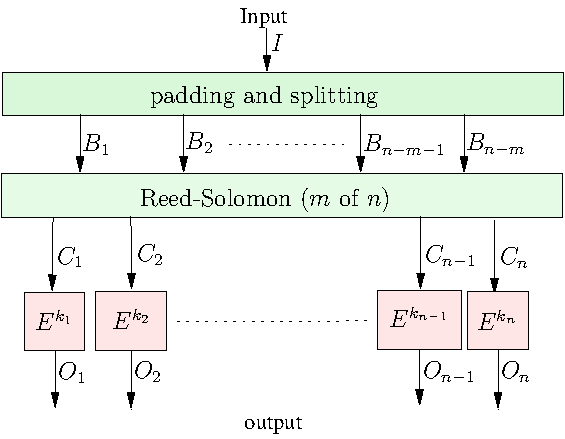
\includegraphics[width=\columnwidth]{inc/addRedundancyOp}
	\caption{Outline of the addRedundancy operation}
	\label{fig:addRedundancyOperation}
\end{figure}
It may be subdivided into the following operations:
\begin{itemize}
	\item Pad the original message block in such a way, that all resulting blocks are a multiple of the block size of the encrypting cypher.
	\item Apply a reed solomon operation in a given GF space with a vanderMonde matrix.
	\item Encrypt all resulting blocks with an unpadded symmetrical encryption.
\end{itemize}


\section{VortexMessage Request Processing}
Vortex message requests allow a Vortex node to gain knowledge about the Vortex network and, create new identities.

\fxwarning{add content here}

\subsection{VortexMessage Requests}
These requests are contained in the header portion of a Vortex message. These requests are purely for bootstrapping and maintaining the quota system and for requesting network capability.

The request information is defined in section \ref{sec:request}. For more information about the exact binary representation of all blocks and data see chapter \ref{sec:spec}.

Any node decides on its own what type of requests are being answered. 

A node not replying to clear text request is called a ``stealth node'' (see \ref{sec:stealthNode}). Such a stealth node discloses itself only to participants which do allready know at least the public key of the node. This usually means that they have ``earned'' this information by issuing a queryPeer request to another node and obtaining the information did already generate costs to the sender.

A node only replying to a fixed set of identities (in that specific case they are not ephemeral) is called a ``hidden node'' (see section \ref{sec:hiddenNode}).

It is recommended that unencrypted requests are not answered. A node may decide to answer unencrypted queryCapability requests in order to enable clients to bootstrap without (or with a minimal) network knowledge.

If a message contains $n$ requests in a header block it must supply at one reply blocks at the beginning of the routing block list. All reply blocks are concatenated and sent using the reply block. If the first block in the routing block list is not a reply block the request will fail.

\subsubsection{QueryCapability Request}
This request is primarily used to initialize a conversation with a node. It contains valuable information about the capability of the node as well as information about the embedding supported or the encryption. A node may or may not reply to a queryCapability requests. Doing so confirms the node to be participating in the vortex network.

The only valid reply is a replyCapability message in encrypted form.

\subsubsection{NewIdentity Request}
If this request is accepted it generates a new ephemeral identity. The identity itself is stored in the header fields. The standard behaviour is to reply with a replyPuzzleRequired block. 

This request generates a temporary ephemeral identity for the limited time denoted in the validity field of the reply block. No quota is assigned during that phase. As soon as the identity offers a valid puzzle solution the requested quota is assigned and the identity may be used for subsequent requests.

If a puzzle is not solved within the given time the temporary identity may be deleted. A node should not accept a solved puzzle after the given duration. 

Request with too high message or transfer quota requests should be answered with an replyPuzzleRequired block containing a zero length puzzle.

\subsubsection{QueryPeer Request}
As outlined in section \ref{sec:request} this request should be very costly and harvesting of known addresses should be hard. Furthermore this request should always  disclose the nodes from a fixed subset of the nodes known to the queried mix. This maximizes the effort to harvest participating nodes.

It is at the same time worth mentioning that this limit may oppose a thread that traffic is concentrated on similar nodes within participating nodes using the same initial set of known addresses to bootstrap. This due to the fact that if using the same node to bootstrap for multiple participants within a group results in peer knowledge which is similar. tThus resulting in a similar network. It is however also worth mentioning that participants belonging to more than one group will evolve over time as their different peer partners will result in different anonymity sets over time even when applying exact the same anr reproducaible rules.

\fxwarning{integrate sec query section from GIT here}

\subsubsection{TransferQuota, MessageQuota,  and QueryQuota Request}
This request may be accepted by a node if and only if the sender is a valid identity. It may be accepted even for a temporary identity.

The transfer quota offers the capability to raise the number of bytes an identity may transfer. This quota may be risen at any time. It is up to the owner of an ephemeral identity and the node using the identity to decide whether an identity may be kept or not respectively its quotas raised.

The Message Quota is a quota not limiting the number of bytes but the number of messages. As every message generates accounting overhead this number has to be limited as well. There are constraints similar to transferQuota when raising this value.

The queryQuota request enables the owner of an identity to query the current amount of remaining messages respectively bytes.

\subsection{VortexMessage Reply Blocks}
Reply blocks are as outlined in section \ref{sec:replyBlock} prefixed payload blocks. All reply blocks except the ctxless\ldots reply blocks are a result of a header request.

\subsubsection{ReplyCapability block}
The replyCapabilityBlock is the reply block to a queryCapability Request. The information provided here is outlined in section \ref{sec:replyBlock}. It is important to note that this block is even when requested in plain is always onionized and thus unreadable for third parties. 

A node may offer different capabilities to known identities than to anonymous clear text requests.

\subsubsection{replyPuzzleRequired block}


The replyPuzzleRequired block is the block reflecting the payment for a requested operation such as newIdentity, queryPeer, transferQuota, or messageQuota request.

Every puzzle block will create an accounting entry as outlined in section \ref{sec:accounting}. 

A node may reject an operation for any reason including exceeding an unnatural ammount of outstanding puzzles.

A reply containing a null length puzzle means that the requested operation is rejected.
                                 i
\fxwarning{This block will change as new proof of work are introduced. The same applies to the respective header section}

\subsubsection{replyStatus block}
\fxwarning{This block will possibly disapear}

\subsubsection{CtxleswhichsNewindentity block}                                                                                                                                            longer in service. It  is done by authenticating with a header block validly authenticating the old identity. It provides a new identity tuple containing a transport layer address and the corresponding ke
Th new identity block is to propagate a newly generated, non-ephemeral identity of a user. This block should not be ignored by any node. It enables a user to strengthen its identity. 
             A node                                                                             e
It is however should ignore the request if its acceptance results in a reduced security lavel of the current identity.


\chapter{Vortex Prerequisites}
\section{Hardware}
No special Hardware is required for running Vortex nodes. The capabilities of Vortex are designed in such a way that ordinary mobile phones may act as vortex nodes. It is however recommended to have a node always connected to the internet. A mobile phone may disconnect from time to time based on the availability of the network. For our experiments we use a RaspberryPi Version 1. It is however recommended to use a faster, newer model due to the memory requirements of the proof of work.

\fxwarning{add more content here}

\subsection{Considerations Regarding Weak or Unsuitable Hardware}
\fxwarning{add more content here}

\section{Addresses}
A Vortex address is built as follows: $vortexAddress=<transport>:<address>!<publicKey>$

To allow storage of Vortex addresses sin standard messaging programs such as Outlook or Thunderbird. We define an alternate representation $encodedVortexAddress=base64(<transport>:<address>).<publicKey>@localhost$. 

The suffix ``@localhost'' makes sure that a message intended for Vortex is not routed by any non-participating server.

The main downside of vortex addresses are that they are no longer readable by a human. The main reason for this is the public key which is required. We may abstract this further by allowing clear text requests on the main email address for the public key. Such requests must then be answered by the vortex account with the valid Vortex address.

\subsection{Public Key Encoding in Address Representation}
The public key of an address is encoded as follows:
\begin{enumerate}
	\item The asymmetric key is encoded as specified in the AsymmetricKey in ASN.1
	\item The ASN.1 representation is then encoded using BASE64
\end{enumerate}	

\section{Transport Layers}                                          P
As transport layer protocols we specified the protocols SMTP and XMMP as valid transport layers. In the following sections we specify the transport properties for these protocols.

\subsection{Embedding Spec}
Messages are always encoded as attachments in SMTP and XMMP. 

If not further specified by the receiving node an attachment should be the encoded message. 

Valid properties may be:
\begin{itemize}
	\item $ plainEncoding="("plain:"<numberOfBytesOfOffset>[,<numberOfBytesOfOffset>]*")$
	\item $ F5Encoding="(F5:"<passwordString>[,<PasswordString>]*")"
\end{itemize}

All nodes responding to clear text should at least support $encoding=plain:0,256$.

\section{Client}
We did not create a Vortex client for sending messages. Instead we used a standard Thunderbird email client pointing to a local SMTP and IMAP Server provided by a Vortex proxy. On the SMTP side Vortex does encapsulate where possible mails into a Vortex message and builds automated route to the recipient. The SMTP part of vortex may be used to encapsulate automatically all messages with a known Vortex identity into a vortex message. On the IMAP side it merges a local Vortex message store with the standard Email repository building a combined view.

Using Vortex like this offers us the advantages of a known client with the anonymity Vortex offers.

This has certain downsides. At the moment the vortex client has only a local store this makes it impossible to handle multiple simulatneously connected clients to use Vortex. This is however just a lack of the current implementation and not of the protocol itself as we may safely use an IMAP storage for storing vortex mails centrally.

\subsection{Vortex Accounts}
By definition any transport layer address may represent a Vortex identity. This fact may make people believe that their current email or jabber address is suitable as Vortex address. This is technically perfectly true, but should not be done for the following reasons:

\begin{itemize}
	\item If an address is identified as a vortex address it may be blocked (directly or indirectly) by an adversary.
	\item If a vortex node is malfunctioning non-vortex messages should remain unaffected. This is more likely to happen if non-Vortex messages are kept in a separate account.
	\item If a user wants no longer to maintain its Vortex address (hopefully there will be a better technology in future) he just may give up his Vortex accounts. If he would have been using his normal messaging account for Vortex he would receive mixing messages which he has to filter in future.
\end{itemize}

\subsection{Vortex Node Types}

\subsubsection{Public Vortex Node}
Public nodes are nodes, which advertise themself as normal mixes. Just as all nodes they may be an endpoint or a mix. Typically they accept all requests exactly as outlined in \ref{tab:protoReplyCrit}. As an immediate result of the publicly available information about such a node the owner may be target of our adversary. Pressure may be oposed to close down such a node. However since we do not need a specific account we may safely close down one transport account and open up a different one. This is even possible on the same infrastructure. To notify other users of the move and remain reachable, a user may send an \fxwarning{incomplete; Where is the contextless update?}

\subsubsection{Stealth Vortex Node\label{sec:stealthNode}}
This node does not answer any clear text requests. As an immediate result the node is only usable by other nodes knowing the public key of this node. The node is therefore on a known secret base only reachable.

\subsubsection{Hidden Vortex Node\label{sec:hiddenNode}}
A hidden node is a special form to a stealth node it has a set of preset identities. Only these entities are processed. This behaveour has certain drawbacks. An identity may not be changed. As an immediate result traffic may become a pseudonymity. To counter this effect at least partially we may use the same local identity for multiple senders. As an immediate result the sender is only one of all senders knowing the private key of an identity.

\chapter{MessageVortex - Transport Independent Messaging anonymous to \nth{3} Parties\label{sec:spec}}
This approach is different from all approaches discussed previously. Unlike them we put complete distrust into the infrastructure being used. Furthermore we do not rely on a custom server infrastructure in the internet. Instead we take advantage of the availability of internet connected devices such as internet connected mobile phones, tablets, or even commonly available SoC such as RaspberryPi or similar. It is still very hard to maintain a server in the internet and considering the vastly growing amount of automated attack carried out against internet connected servers it is not advisable or realistic to assume that a future user of this system owns either a server or connects to a service which is offering explicitly anonymizing services. These infrastructures would be suspectible to monitoring or even banning. Instead we take a different approach.

We use common messaging protocols as transport layers and connect to them using the respective client protocols. The actual mixes are operated by the users on their ``always connected'' devices. It goes without saying that such a system is far less reliable than a traditionally run server as this hardware is typically cheap and normally connected to the internet using a bandwidth shared media.

The basic idea is that a client generates all traffic (including decoy and diagnosis) by itself. It defines the routes a message takes through the mixes and decides which targets are receiving dummy traffic at the same time. In such a system, even when possessing all the nodes routing the traffic (without the endpoints) an anonymity set of $k$ (whereas the size of $k$ is defined by the sender) is guaranteed.

As decoy traffic is generated with the same operations as the true content is split it is impossible for an adversary running a node to determine whether he is generating noise or actually processing the true message.
All nodes, regardless of endpoint or mix implement the same logic and fulfil the same functions which makes it impossible to deteremine the function. Exit nodes as in Tor or similar systems do not exist.


%\fxwarning{add a lot more text here}
%\begin{figure*}[h]
%	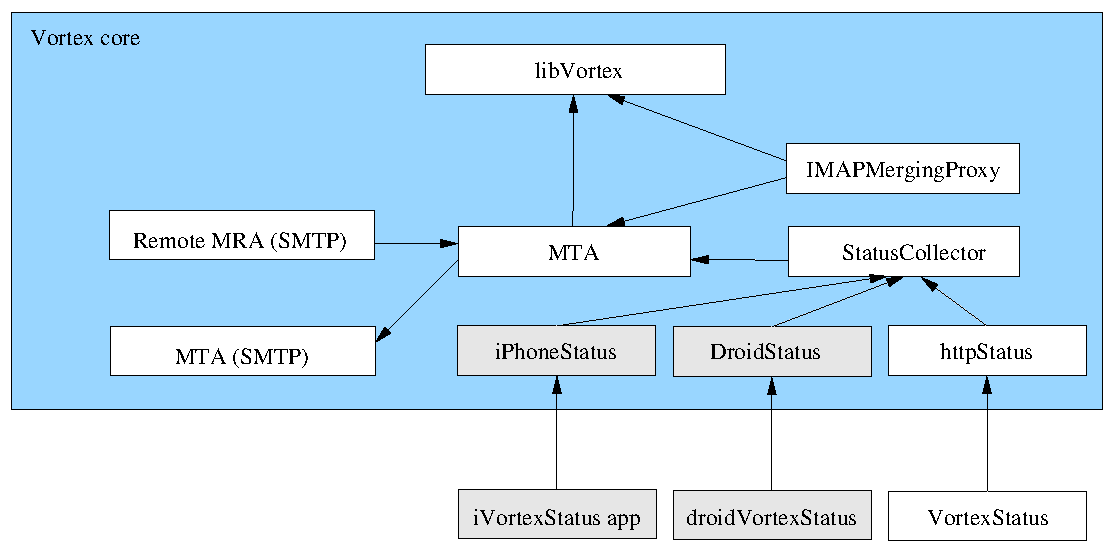
\includegraphics[width=\textwidth]{inc/VortexModules.pdf}
%	\caption{Overview of the Vortex modules}
%	\label{fig:vortexModules}
%\end{figure*}
%\fxwarning{replace image with up to date representation; show implemented and not implemented parts; Maybe make it two column wide}
%

\section{Accounting}
In table \ref{tab:protoReplyCrit} we show under what circumstances a reply to a header request should be sent. The capitalised words MAY, MUST, SHOULD and SHOULD NOT are used as defined in RFC2119\cite{RFC2119}.
\begin{table*}[h]
	\centering\scriptsize
	\begin{tabular}{|l|l|l|l|l|}\hline
		\diaghead{\theadfont Request Criteria}{Request}{Criteria} & \thead{unknown identity; cleartext} & \thead{unknown identity; encrypted} & \thead{expired identity; encrypted} & \thead{known identity; encrypted}\\\hline
		newIdentity	 	& SHOULD NOT 	& SHOULD NOT& Invalid (Error) 	& Invalid (Error)\\              
		queryPeer       & MUST NOT      & MUST NOT  & MAY               & MAY\\        
		queryCapability	& SHOULD 		& MUST 		& MUST				& MUST \\
		messageQuota	& MUST NOT 		& MUST NOT	& MAY				& MUST \\              
		transferQuota	& MUST NOT		& MUST NOT	& MAY				& MUST \\\hline             
	\end{tabular}	
	\caption{Requests and the applicable criteria for replies}
	\label{tab:protoReplyCrit}
\end{table*}

\section{Routing}

\fxwarning{add text here and state machine of message}



\fxwarning{add content here}

\section{Blending layer}
Blending layer must be crafted in a careful manor. A blending layer is responsible for sensible content generation of the transport media plus embedding a VortexMessage into the transport layer according to specs provided by the original sender.

The original sender has no control over the plain text messages to avoid possibilities of sending targeted messages over the transport layer using MessageVortex. This differentiates MessageVortex from other systems having ``exit nodes'' such as tor.

\fxwarning{add parrot circumvention}

\subsection{Plain Inclusion}
The data stream has of the MessageVortex protocol has no structure visible from the outside. This property allows embedding as structureless information in files with a similar entropy. We did an analysis on common file formats in the internet to figure out which file format is suitable for this type of inclusion.

It is improtant to understand that this is very weak form of information hiding. A human observer may easily tell ``real'' data from ``broken'' data apart. A human is not able to tell whether a file is seriously broken or contains a VortexMessage.

\subsubsection{File Type Candidates}

We were unable to find any scientifical data regarding what type of traffic or attachment is common in the internet. We therefore tried to analyze mail logs (smtp) of a mail provider. We were scanning $567594$ emails for attachment properties after the spam elimination queue. $16.5\%$ of all scanned messages had an attachment. The top 20 attachment types distributions are shown in \ref{tab:emailAttachments}.
\begin{table}[H]
%	\centering\scriptsize

\begin{tabular}{l|r}\hline
	Type																		& \%\\\hline
	image/jpeg                                                                  &	27.4\\
	application/ms-tnef	                                                        &	13.7\\
	image/png                                                                   &	13.3\\
	application/pdf                                                             &	10.7\\
	image/gif                                                                   &	7.4\\
	application/x-pkcs7-signature                                               &	5.4\\
	message/rfc822                                                              &	7.0\\
	application/msword                                                          &	3.1\\
	application/octet-stream                                                    &	3.0\\
	application/pkcs7-signature                                                 &	2.3\\
	application/vnd.\ldots.wordprocessingml.document	                        & 	1.4\\
	message/disposition-notification                                            &	1.1\\
	application/vnd.ms-excel                                                    &	0.8\\
	application/vnd.\ldots.spreadsheetml.sheet                                  &	0.6\\
	application/zip                                                             &	0.5\\
	application/x-zip-compressed                                                &	0.5\\
	image/pjpeg                                                                 &	0.4\\
	application/pkcs7-mime                                                      &	0.4\\
	video/mp4                                                                   &	0.4\\
	text/calendar                                                               &	0.4\\\hline
\end{tabular}
	\caption{Distribution of 20 20 attachment types}
\label{tab:emailAttachments}
\end{table}
                     about implementation 
As expected the amount of images within mail was very high ($\approx 50\%$). Unfortunately we were unable to analyze the content of ms-tnef attachments retrospectively. It seems that based on this figures information hiding within images in email traffic is a good choice.

\subsection{F5 Steganography}

\fxwarning{add content here}

\section{Message Flows}

\fxwarning{add content here}

\section{Considerations for Building Messages}
In a worst case scenario we assume that an adversary is controlling most of the network utilized for anonymisation. While this is not necessarily a problem (as pointed out earlier) it allows an adversary to track a message while agents are being used under his control. So for simplicity and as a worst case assumption we always assume that an adversary has perfect knowledge of an associated message flow. This is however a worst case scenario. One missing agent disconnects the whole chain and as messages are not traceable in size.

\fxwarning{add selffailing operations as checkpoint}

\subsection{Ephemeral identities}
\fxwarning{expiring ephemeral identities should not only be replaced after their expiration but anytime during the livetime}

\subsection{Timing of messages}
\fxwarning{add content here}

\subsection{Diagnostics}
\fxwarning{add content here}

\fxwarning{add here why is there no hashing operation (makes traffic distinguishable)}


\subsubsection{Implicit Diagnostic}
\fxwarning{Add comments about messages splitting and returning to sender}

\subsubsection{Automatic Explicit Diagnostic}
\fxwarning{Add comments about error and diagnosis messages officially spliting of messages}
                                        the following
\subsubsection{On-Demand Explicit Diagnostic}
\fxwarning{Add comments about normal, error, and diagnosis messages being picked up by a routing block}

\fxwarning{list all requirements}



\section{Verification of requirements}
In the previous sections we identified a list of requirements.

In the following subsections we will iterate through all requirements and verify to what degree we achieved the goal.

\paragraph*{\ref{req:zeroTrust}:} 
We have not put any trust into an external infrastructure. While we do assume that all routing nodes act as defined. A misbehaving node may be identified and eliminated without putting any trust on other nodes. Analysis have shown no means for a misbehaving node which might be intentional or unintentional endangering anonymity at any time. We do not rely on any third party technology or infrastructure for our anonymity. 

This requirement is therefore fulfilled.

\paragraph*{\ref{req:P2P}:} 
No node has additional privileges or offers additional services. All are equal and share the same privileges.

This requirement is therefore fulfilled.

\paragraph*{\ref{req:untagable}:} 
Messages may not be tagged. All content is either strictly onionised or defined and linked with unknown hooks. Tampering with a message will cause the message delivery to fail at the next node.

This requirement is therefore fulfilled.
 
\paragraph*{\ref{req:unbugable}:} 
There are always means to bug a message. As we put trust in sender and recipient and we know already that a intermediate mixing node is not able to modify the message the protocol is hard to bug. There may be a possibility to bug a message with a routing log entry over DNS. If a recipient is not resolving names or trusts in the content of such a message he is safe.

This requirement is therefore fulfilled. May be only partially fulfilled if log entries are not handled with care.

\paragraph*{\ref{req:replay}:} Messages may only be replayed a limited amount of times. The number of replays is controlled by the sender and may not be altered by any mix. A malfunctioning mix replaying more often than allowed will not be able to extract any information than the information it obtained when sending the first time. 

This requirement is therefore fulfilled.

\paragraph*{\ref{req:accounting}:} 
All identities generated are not traceable as any identity is generated without any context and may not be mapped to an older or newer identity (perfect anonymous forward identity). Neither the source nor the replies may be used to be traced as all messages 

This requirement is therefore fulfilled.

\paragraph*{\ref{req:anon}:} This point is the hardest to proof. We certainly achieved a high degree of anonymity. No node can tell by observing traffic if a node is a final recipient or just a mix. There are however some weaknesses in the protocol. As the implementation is currently connecting simultaneously to the true name (email or jabber account in the current implementation) and the Vortex account the user might be identified by that fact. Using a anonymisation proxy could solve the problem but it would violate the Zero trust principle.

This requirement is therefore only partially fulfilled. However, the weakness is very faint.

\paragraph*{\ref{req:boot}:} 

\fxwarning{add content}
\paragraph*{\ref{req:cryptVar}:} 

\fxwarning{add content}

\paragraph*{\ref{req:easy}:}

\fxwarning{add content}

\section{Considerations for Routing Messages}
\subsection{Time of sending}
Messages should always be sent timewise nearby other messages. This means that the best moment for sending a message in a ready queue is at a time when sending of other messages is due. However no optimisation should be done to send as many messages as possible at the same time. this would lead to a forseeable behaviour of the routing layer and thus to misusable behaviour.

\section{Real World Considerations}
This approach is heavily dependent of the transport protocol and builds on top a new obfuscating/routing layer. For this system to become a real peer-to-peer approach some additional quirks are required. A message-Vortex-Account needs always an active routing handler. This routing handler may be introduced by new server capabilities or by having a device handling the routing from the client side. For this reason we built a RaspberryPi appliance capable of connecting to one (or more) accounts fetching incomming mails, analysing them and reroute them if necessary. Although the system is designed to be run on a RaspberryPi the software might be installed to any Java capable client. The RaspberryPi is just one affordable lightweight device which offers all required capabilities.

\subsection{No Routing Log}
There was up until very late a routing log functionality in the protocol. This functionality did however have the disadvantage that it allowed bugging and could possibly  disclose intermediate mixes to a recipient which did not comply with the policy the mixes might have chosen. Therefore this feature was dropped and replaced with the fetch block behaviour.

\subsection{No Verification Possibilities}

\subsection{Very Limited Control Blending Layer for the sending node}

\subsection{Message Content}
\fxwarning{add content here}

\chapter{Security Analysis}
In the following sections we emphasize on attacks targeting either sender recipient tuples or on identification of participants. 

Based on the protocol we may safely assume the following key ponts:
\begin{itemize}
	\item An adversary knows and controls a significant number of nodes (for our analysis we assume less than 80\%).
	\item An adversary may observe the traffic at any point without getting any information about the message content
	\item An adversary is not capable of matching multiple messages on different nodes to one message.
\end{itemize}

We always assume an adversary to have more knowledge than we think he may extract from the messages.
\begin{itemize}
	\item We assume that an adversary knows all messages of a transaction running over his nodes and matches them correctly to the same message.
	\item 
\end{itemize}

We assume that the adversary is targeting the following informations:
\begin{itemize}
	\item Sender identity
	\item Recipient identity
	\item Message content
	\item Message size
\end{itemize}

Attacks on the users identity atre no longer possible as the identity used on the nodes is based on ephemeral identities instead of the users true identity. As the ephemeral identities may exist in parallel, overlapping or in a serial manor and are strictly unlinked to the true identity no statement can be made concerning the linking of ephemeral identities to the true identities. Frequency patterns or behavioral patterns may be split among multiple identities and distributed over multiple nodes. 

Frequency and bandwidth analysis are not possible as frequency and bandwith of a single message is not trackable and the size of a message is generally not related to the message flow. An exception to this statement is when routing a different message through a vortex system using a reused routing block general statements such as ``the message is bigger than the previous one'' about the messages size is possible if the routing block makes use of relative split operations. In experiments, we were able to mimic any desired communication pattern we wanted for an adversary to be found.

The message content remains cryptographically secured if the dual trust (sender and receiver node) is not broken, the message is encrypted on the senders node, the message is only decrypted on the receivers node, and remains at least wrapped in this encryption during the whole transfer. 

\subsection{Attacking Routing Blocks}
\fxwarning{add content here; Routing block length analysis}

\section{Attack on Message size}

\fxwarning{add content here}

\chapter{Additional Considerations}
\section{Man in the Middle Attacks to Conversations}

\fxwarning{add content here}

\section{Identification of Participating Nodes}

\fxwarning{add content here}

\subsection{Identification by Content}
It is possible to identify a message by content. Assuming that an adversary knows the applied blending method he may identify an ASN.1 structure of \fxerror{incomplete}

\fxwarning{add content here}

\subsection{Identification by Query}

\fxwarning{add content here}

\subsection{Identification by Traffic Type}

\fxwarning{add content here}

\subsection{Identification by Bandwidth}

\fxwarning{add content here}

\subsection{Identification by Behavioural Analysis}

\fxwarning{add content here}

\section{Storage of Messages and queues}
The storage of messages sent though MessageVortex should be handled with great care. It seems on the first sight a good idea to merge all messages in a globally available storage such as the IMAP account of the receiving entity. However -- In doing so we would discover the message content to the providing party of a mail account. Since we handled the message with great care and tremendous costs up until this point it would be careless doing so. 

Storing them in a localized and receiving entity controlled storage is definitely a good idea but leaves security considerations like a backup possibly to an end user. This might be better, but in effect a questionable decision. There is however a third option. By leaving the message unhandled on the last entity of the MessageVortex chain we may safely backup the data without disclosing the message content. Merging the content then dynamically through a specialized proxy would allow the user to have a unified view on his without compromising the security.

\fxwarning{implemented in prototype?}

